
\documentclass[a4paper,12pt]{article} 
\usepackage[top = 2.5cm, bottom = 2.5cm, left = 2.5cm, right = 2.5cm]{geometry} 
\usepackage[T1]{fontenc}
\usepackage[utf8]{inputenc}
\usepackage{multirow} 
\usepackage{amsmath}
\usepackage{amssymb}
\usepackage{booktabs} 
\usepackage{graphicx}  
\usepackage{subfig}
\usepackage{setspace}
\setlength{\parindent}{0in}
\usepackage{float}
\usepackage{tablefootnote}
\usepackage{fancyhdr}
\usepackage[english]{babel}
\usepackage{xcolor}
\usepackage{multirow}
\usepackage{listings}
\usepackage{dcolumn}
\lstset{
  basicstyle=\footnotesize\ttfamily,
  columns=fullflexible,
  frame=single,
  breaklines=true,
  postbreak=\mbox{\textcolor{red}{$\hookrightarrow$}\space},
}
\usepackage{hyperref}
 \hypersetup{
     colorlinks=true,
     linkcolor=black,
     filecolor=black,
     citecolor = black,      
     urlcolor=blue,
     }
\usepackage{csvsimple}
\pagestyle{fancy} 
\fancyhf{} 
\lhead{\footnotesize Economics 714: PS2}
\rhead{\footnotesize Javier Tasso} 
\cfoot{\footnotesize \thepage} 




\begin{document}





\begin{tabular}{p{15.5cm}} 
{\large \bf Economics 714 - Computational Methods in Economics} \\
University of Pennsylvania \\ Fall 2021 \\ \\ 
\hline 
\\
\end{tabular} 

\vspace*{0.3cm} 

\begin{center} 
	{\Large \bf Problem Set 2} 
	\vspace{2mm}
	
        
	{\bf Javier Tasso} 
		
\end{center}  

\vspace{0.4cm}

%%%%%%%%%%%%%%%%%%%%%%%%%%%%%%%%%%%%%%%%%%%%%%%%
%%%%%%%%%%%%%%%%%%%%%%%%%%%%%%%%%%%%%%%%%%%%%%%%



    % Exercise 1    
    
     
    \section{Steady State} 
    \medskip
    
    With $z=0$ the resource constraint of the economy reads as follows. 
    
    \begin{align} \label{consumption_equation}\begin{split}
        c + i & = k^{\alpha}  l^{1-\alpha} \\ c + k' - (1-\delta) k & = k^{\alpha}  l^{1-\alpha} \\ c & = k^{\alpha}  l^{1-\alpha}  - k' + (1-\delta) k \end{split}
    \end{align}
    
    Given the state $k$, the social planner chooses $l$ and $k'$ (and $c$) to solve the following problem. 
    
    \begin{align*}
        V(k) & = \max_{k',l} \bigg\{(1-\beta)\bigg(\ln[k^{\alpha}  l^{1-\alpha}  - k' + (1-\delta) k] -\frac{l^2}{2}\bigg) + \beta V(k')\bigg\}
    \end{align*}
    
    Take first order condition with respect to labor to get the following intratemporal equation. 
    
    \begin{align}\label{intratemporal_equation}
        \frac{1-\alpha}{c} \cdot \bigg(\frac{k}{l}\bigg)^{\alpha} & = l
    \end{align}
    
    Take first order condition with respect to capital in next period and use the envelope theorem to get the following intertemporal equation. 
    
    \begin{align}\label{intertemporal_equation}
        \frac{1}{c} =  \frac{\beta}{c'} \cdot  \bigg[\alpha \bigg(\frac{l'}{k'}\bigg)^{1-\alpha} + 1 - \delta \bigg]
    \end{align}
    
    Set $c=c'=c_{SS}$, $l=l'=l_{SS}$ and $k=k'=k_{SS}$ and use equations (\ref{consumption_equation}), (\ref{intratemporal_equation}) and (\ref{intertemporal_equation}) to find the steady state values. For $\alpha = 0.33$, $\beta = 0.97$ and $\delta = 0.1$. Table (\ref{SteadyStateValue_Table}) shows the values in the steady state. 
    
    
    
    \begin{table}[!htbp]
        \centering
        \caption[Short Caption for LoT]{Steady State Values}\label{SteadyStateValue_Table}
    \csvautotabular{econ714_homework2_question1_output.csv} 
    \end{table}

    

     
    
    % Exercise 2   
    
    \medskip
    \medskip
    \section{Value Function Iteration with a Fixed Grid}     
    \medskip
    
    Figure (\ref{value_and_policy_function}) plots the value and policy functions and it includes information about the number of iterations, time elapsed and tolerance level. Figure (\ref{response_to_tech_shock}) plots trajectories after the following shock: initially we are in the steady state when $z=0$, suddenly there is a positive shock, that is, $z_1=0.05$ and after that shock $z_t=0$ forever for $t>1$. 
    
    \begin{figure}[!htbp]
        \centering
       \subfloat{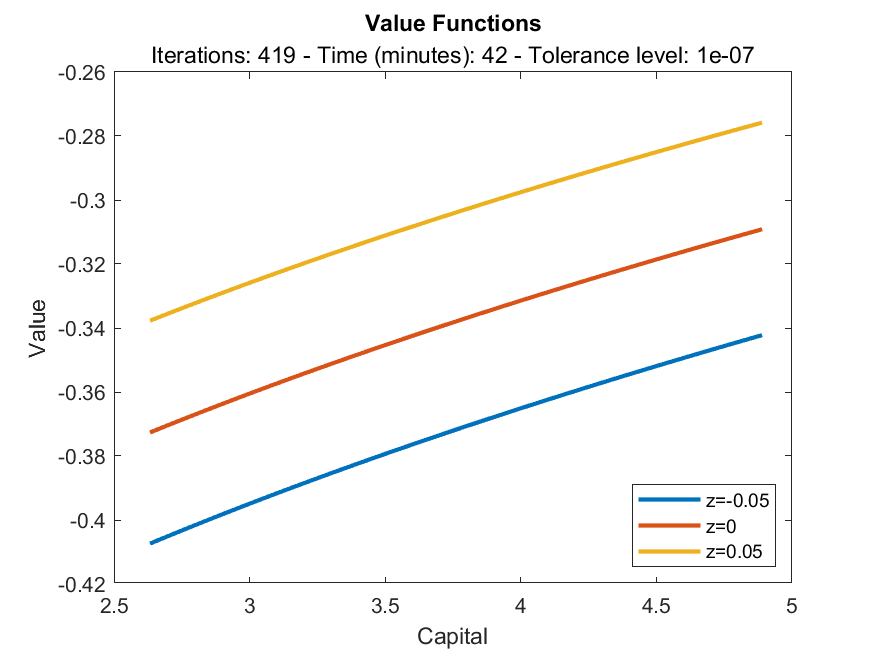
\includegraphics[scale=0.5]{econ714_homework2_question2_plot_value_function.png}}
       \subfloat{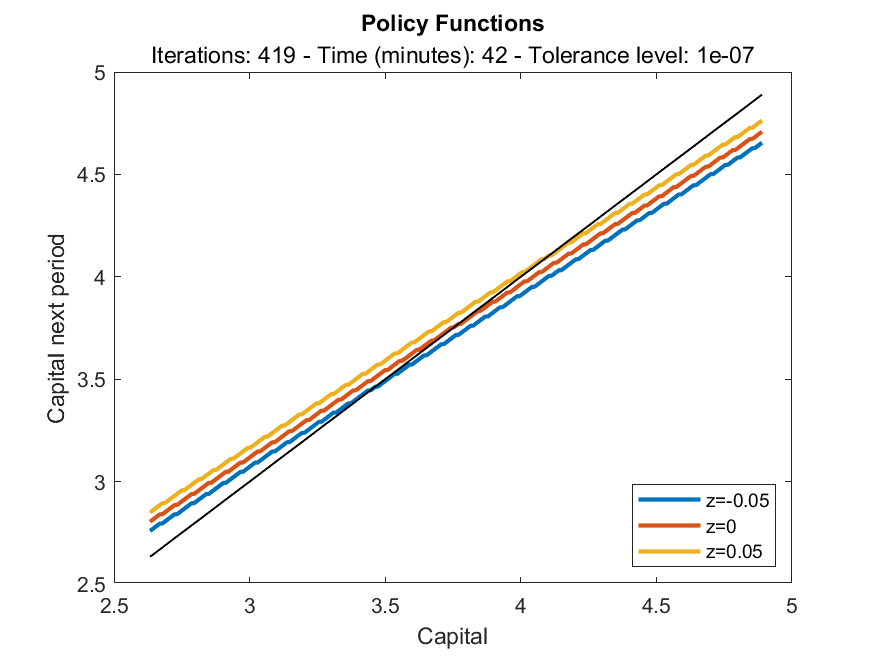
\includegraphics[scale=0.5]{econ714_homework2_question2_plot_policy_function.png}} 
       \caption{Value and Policy Functions - Fixed Grid}
       \label{value_and_policy_function}
   \end{figure}
    
    \begin{figure}[!htbp]
        \centering
       \subfloat{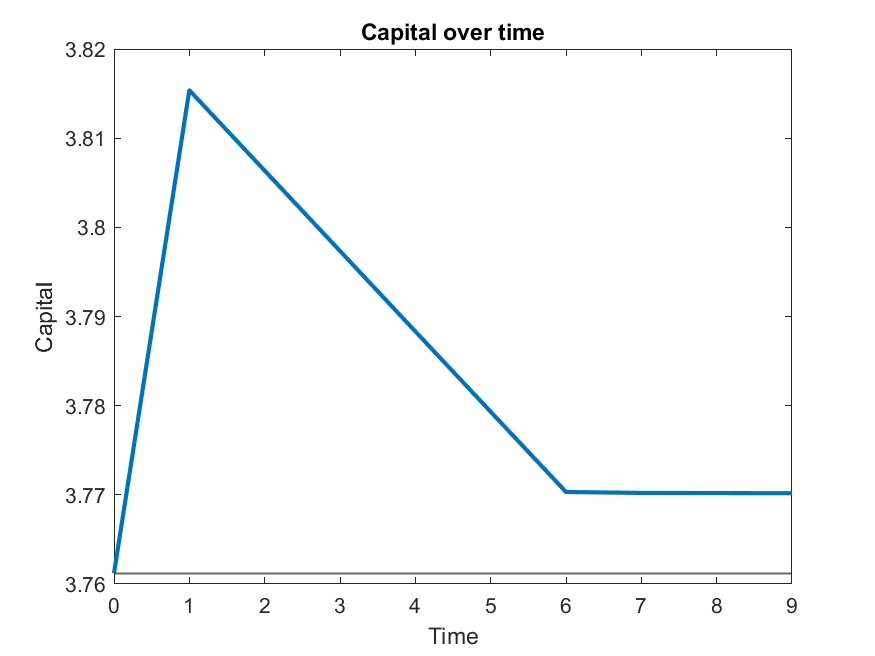
\includegraphics[scale=0.5]{econ714_homework2_question2_plot_capital.png}}
       \subfloat{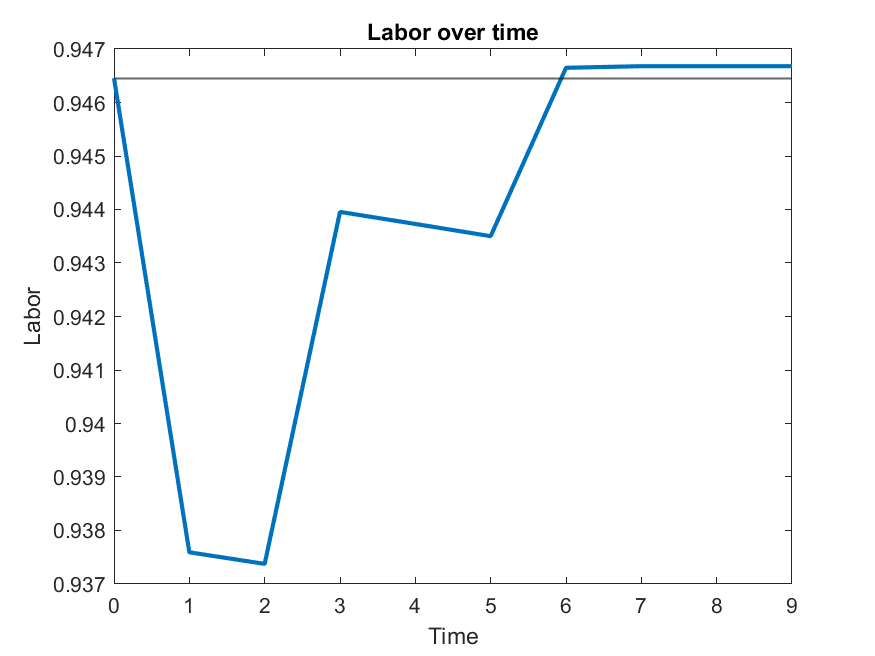
\includegraphics[scale=0.5]{econ714_homework2_question2_plot_labor.png}}
       
       \subfloat{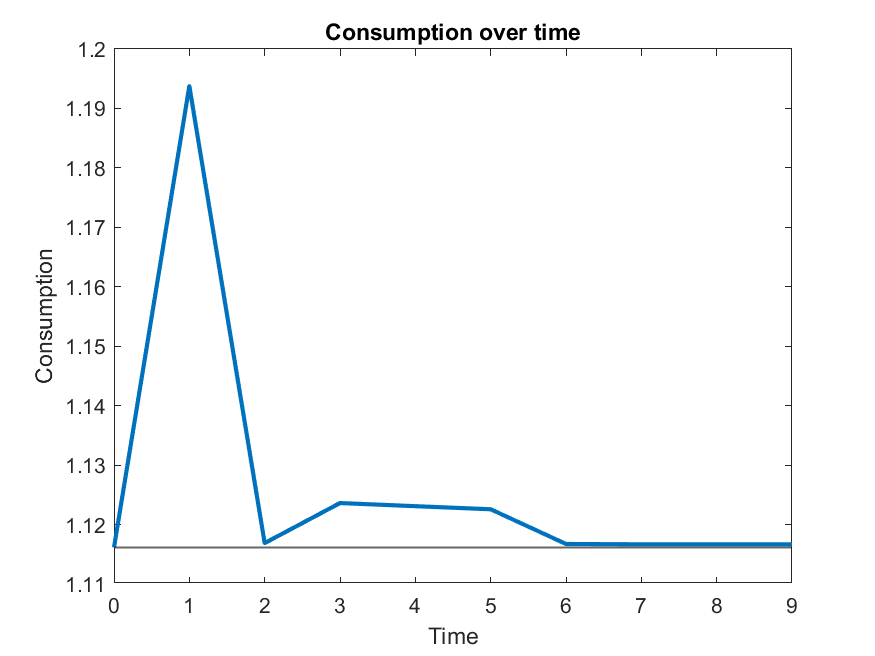
\includegraphics[scale=0.5]{econ714_homework2_question2_plot_consumption.png}}
       \subfloat{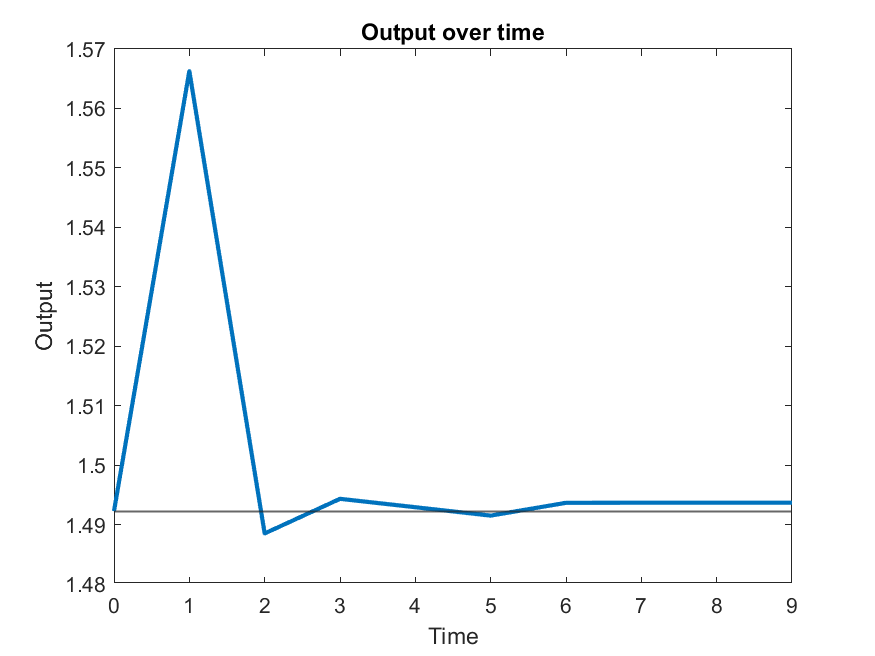
\includegraphics[scale=0.5]{econ714_homework2_question2_plot_output.png}}
        \caption{Responses to a Technology Shock} 
        \label{response_to_tech_shock}
    \end{figure}
    
    % Exercise 3 
    
    \medskip
    \medskip
    \section{Accelerator}     
    \medskip
    
    It does not work. I tried different things. I think I understand how the procedure is, so let me try to describe it briefly. Script \textit{Econ714\_hw2\_1\_VFI.m} has one section where I tried to implement the accelerator.  
    
    % Ideas 
    
    % \begin{itemize}
        % \item Do grid search in the 9 steps where we do not do the max and interpolation. 
        
        % \item Require some iterations doing the max so that the policy function is well behaved. 
        
        % \item What happened first is that the policy function gave me values way too big of capital and then the value function went to negative infinity. 
        
        % \item Now what is happening is that the policy function is a constant. 
        
        % \item Maybe it is because I am not doing linear interpolation and the grid is small. I have to try again with linear interpolation.
        
        % \item Update. It seems to converge now. But it does not finish. It does not accelerate anything. 
        
         %\item Maybe linear interpolation solves the problem. 
    % \end{itemize}
    
    \begin{itemize}
        \item First the algorithm starts as a simple value iteration during the first $50$ iterations. This is not necessary but maybe this is good to get a better guess and to start accelerating when you are close enough. 
        
        \item After that, every $10$ iterations do exactly as before. 
        
        \item On the other $9$ iterations implement something similar to equation $(3)$ of Heer, B., \& Maussner, A. (2008) that we describe as follows. 
        
        \begin{align}\label{to_implement_acc}
            \mathbf{v} = \mathbf{u} + \beta Q \bar{\mathbf{v}}
        \end{align}
        
        \item Vector $\mathbf{v}$ is a vector of one column that stacks together all the values of the grid for the three levels of productivity. With a grid of length $100$ this vector has a length of $300$. Vector $\mathbf{u}$ does the same thing but for the period utility level given $(k,z)$. Matrix $Q$ has zeros everywhere except on those points where the grid of capital is equal to the value of the policy function. Finally vector $\bar{\mathbf{v}}$ is a linear combination of $\mathbf{v}$ of the same size. What this vector does is that it calculates the expected value function using the transition probabilities. 
        
        \item What we want to do in these steps is to solve $(\ref{to_implement_acc})$ for $\mathbf{v}$ and use that as our value function in those iteration. This should speed up things relative to the previous question. 
    \end{itemize}    
    % Exercise 3 
    
    \medskip
    \medskip
    \section{Multigrid}     
    \medskip
    
    %I think this one should be easier because I won't do any interpolation. Just double loop (over current and future capital), compute the optimal level of labor and gridsearch in the capital. 
    
    %\begin{itemize}
        %\item Step 1. Only 100 until it converges. 
        
        %\item Step 2. Now 1000 points until it converges. 
        
        %\item Step 3. Now 10000 points and we are done. 
    %\end{itemize}
    
    %It works and it takes three hours. I can let it run one night to add the number of iterations in the csv. Maybe I can modify the code to do parfor in the last iteration, but this is not a priority.
    
    In the last grid the initial guess that came from the previous grid was so good that it only took one iteration. Figure (\ref{value_and_policy_function_multigrid}) plots the results using multi-grid. It took three hours to run. Figure () compares the value function using the multi-grid to the one we got in question $2$.
    
    \begin{figure}[!htbp]
        \centering
       \subfloat{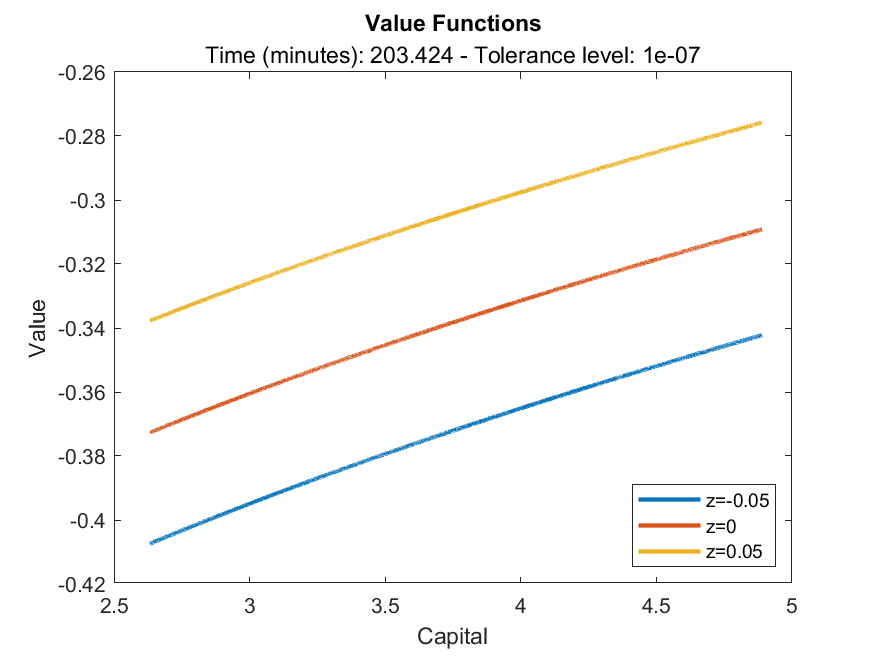
\includegraphics[scale=0.5]{econ714_homework2_question4_plot_value_function.png}}
       \subfloat{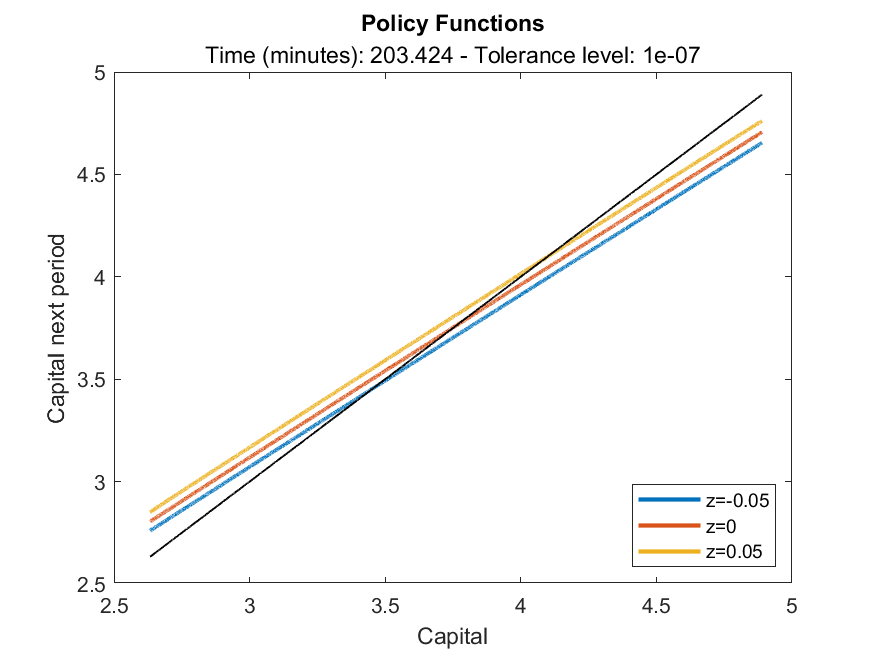
\includegraphics[scale=0.5]{econ714_homework2_question4_plot_policy_function.png}} 
       \caption{Value and Policy Functions - Multigrid}
       \label{value_and_policy_function_multigrid}
   \end{figure}
   
     \begin{figure}[!htbp]
       \centering
       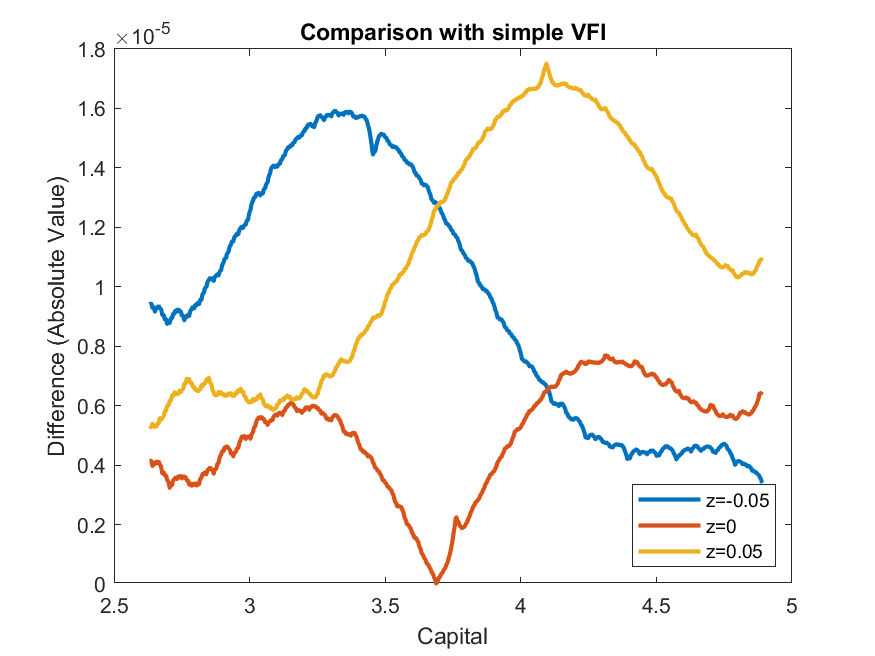
\includegraphics{econ714_homework2_question5_plot_comparison_q2.png}
       \caption{Multigrid vs Simple VFI}
       \label{comparsion_with_VFI_q2}
   \end{figure}
    
    
    \section{Chebyshev}
    
    Just in case here is the problem and the first order conditions. 
    
    \begin{align*}
        V(k,z) & = \max_{k',l, c} \quad \bigg\{(1-\beta) \bigg[\ln(c) - \frac{l^2}{2}\bigg] + \beta \sum_{z'} V(k',z') \mathbb{P}[z'|z]\bigg\} \\ & \quad\quad\quad c=e^z k^{\alpha} l^{1-\alpha} + (1-\delta) k - k'
    \end{align*}
    
    First order conditions are given as follows. We will use these equations to compute several variables of interest. In particular given $(k,l)$ (and production) the intratemporal condition (first equation of (\ref{FOCC})) is going to help us figure out the value of consumption and the Euler equation (second equation of  (\ref{FOCC})) is what we use to find the appropriate coefficients of the Chebyshev approximation. 
    
    \begin{align}\label{FOCC}\begin{split}
        (\text{FOC})_{l}\quad &  \frac{1-\alpha}{c}\cdot e^z \bigg(\frac{k}{l}\bigg)^{\alpha}  = l \\ (\text{FOC})_{k'} \quad &  \frac{1}{c} = \beta \cdot  \mathbb{E}\bigg[\frac{1}{c'}\cdot \bigg(\alpha e^z \bigg(\frac{l'}{k'}\bigg)^{1-\alpha} + 1 - \delta \bigg)\bigg| z\bigg]\end{split}
    \end{align}
    
    Figure (\ref{value_and_policy_function_chebyshev}) shows the value and policy functions, figure (\ref{EEE_chebyshev_pol}) show the Euler equation errors of the approximation and finally figure (\ref{comparsion_with_VFI_q2}) compares this solution with the one we got in question $2$. We do linear interpolation to do the comparison. 

    \begin{figure}[!htbp]
        \centering
       \subfloat{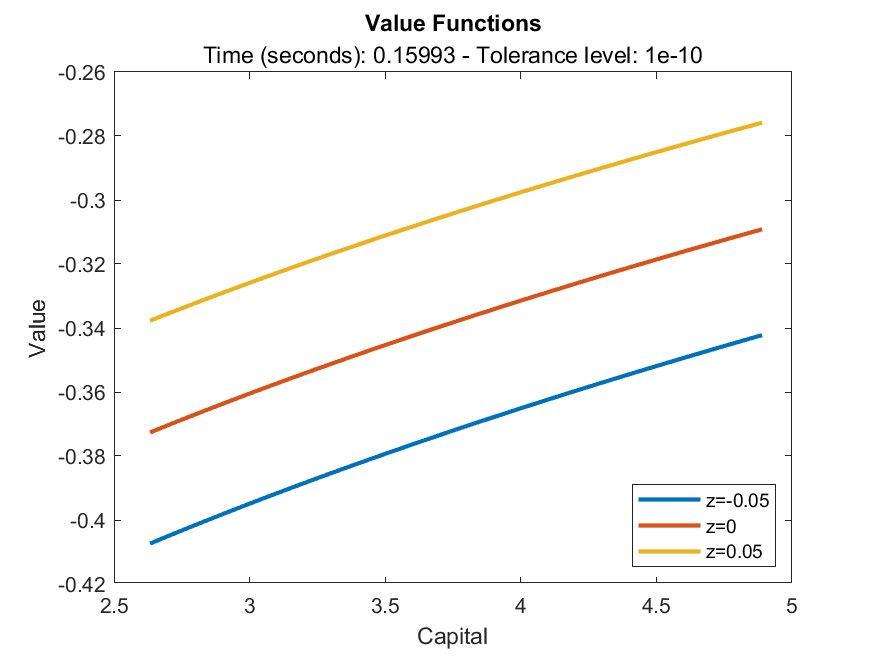
\includegraphics[scale=0.5]{econ714_homework2_question5_plot_value_fun.png}}
       \subfloat{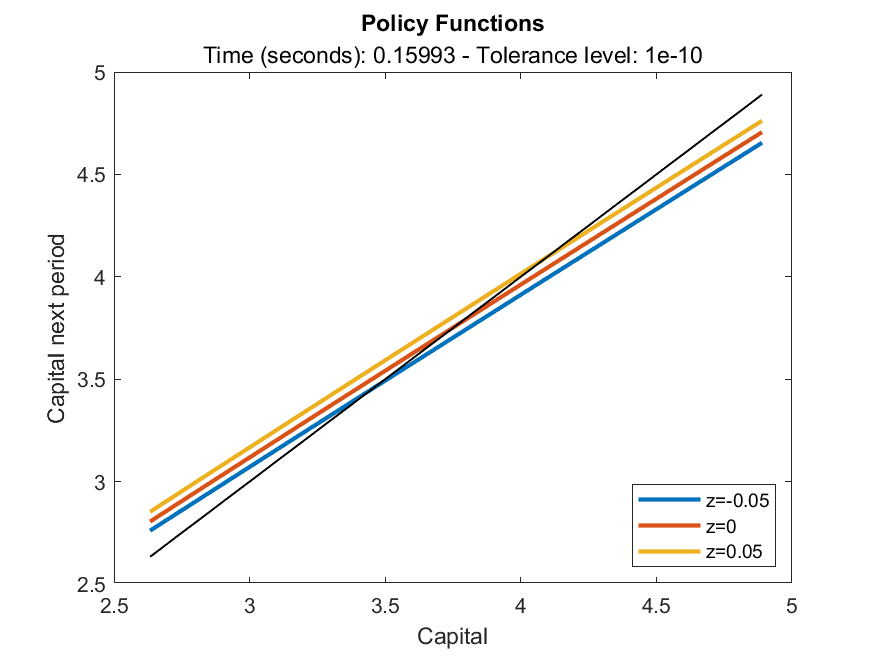
\includegraphics[scale=0.5]{econ714_homework2_question5_plot_pol_fun.png}} 
       \caption{Value and Policy Functions - Chebyshev Polynomials}
       \label{value_and_policy_function_chebyshev}
   \end{figure}
   
   \begin{figure}[!htbp]
       \centering
       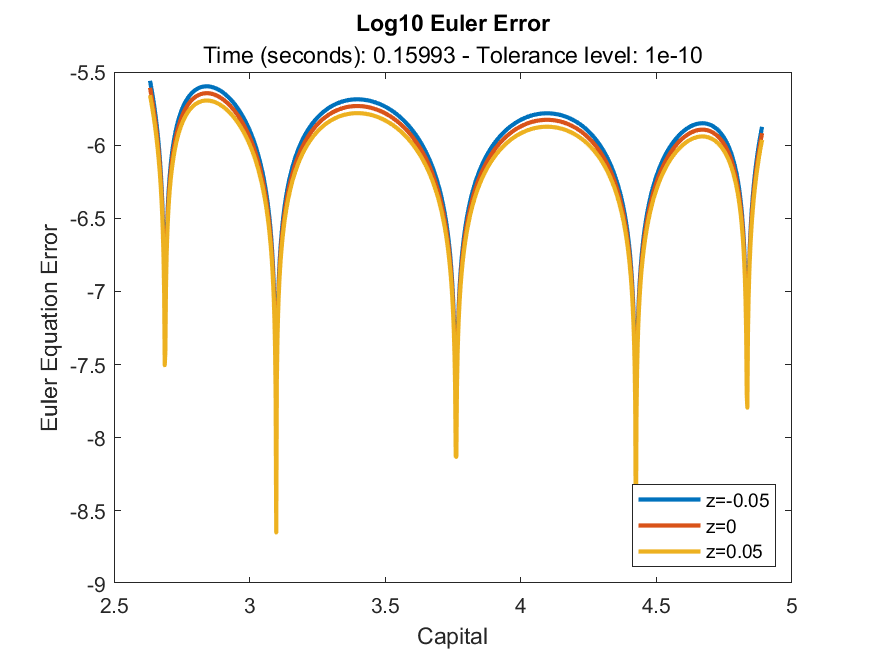
\includegraphics{econ714_homework2_question5_plot_eee.png}
       \caption{Euler Equation Errors - Chebyshev Polynomials}
       \label{EEE_chebyshev_pol}
   \end{figure}
   
  \begin{figure}[!htbp]
       \centering
       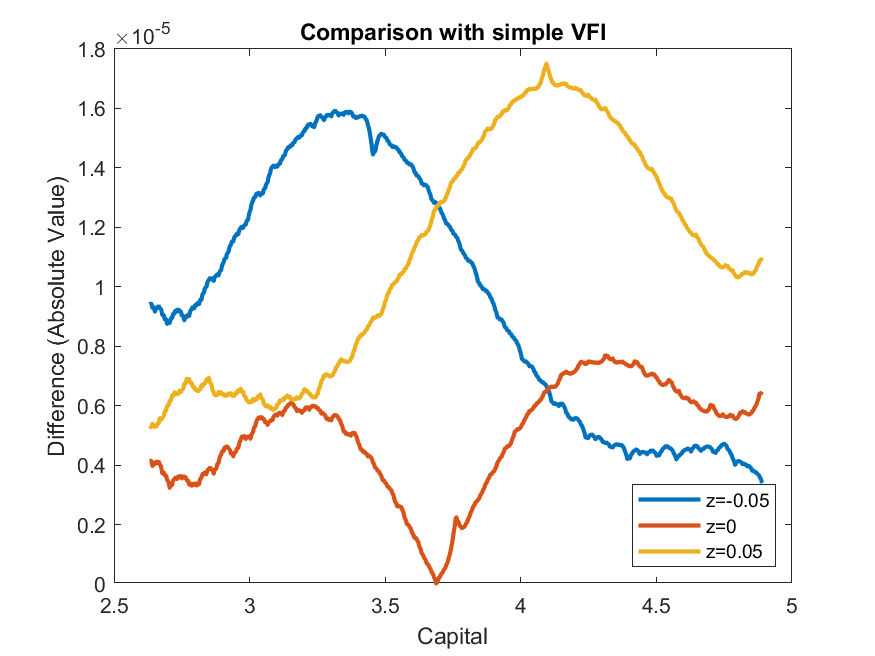
\includegraphics{econ714_homework2_question5_plot_comparison_q2.png}
       \caption{Comparison with simple VFI}
       \label{comparsion_with_VFI_q2}
   \end{figure}
   
   Here we briefly describe the methodology. 
   
   \begin{itemize}
       \item Script \textit{Econ714\_hw2\_2\_Chebyshev.m} does the computation and generates the plots. 
       
       \item Function \textit{residual\_fcn\_2.m} does most of the job. We tried to modify the original code  \textit{residual\_fcn.m} to adapt it to this problem. Given a set of coefficients stored in vector $\rho$ this function calculates the policy function for labor, takes advantage of the first order condition to get consumption and capital next period and repeat the process one more time to construct the residuals. Remember that for the residuals we need information about the current period and next period. After that it calculates the residuals which will depend on $\rho$. 
       
       \item Finally the main script finds $\rho$ such that the residuals are zero and with this choice $\rho^*$ we can compute the policy and value functions. 
   \end{itemize}
   
   \section{Finite Elements}
   
   I try to follow McGrattan, E. R. (1996). My idea is to solve the system given by equation ($15$) in that paper. Let $\text{E}$ be the number of elements and $z$ the productivity shock (remember there are three of them). 
   
   \begin{align}\label{solve_for_theta}
       \sum_{j=1}^8 \int_{k_j}^{k_{j+1}} \vec{w(k)}_{\text{E}} \cdot R(k, z, \theta) dk = 0   
   \end{align}
   
   \begin{itemize}
    
        \item Function \textit{weight\_fun\_capital.m} has inputs $(k, \mathbf{k}_{\text{ELEMENTS}})$ where $k$ is a state of capital and $\mathbf{k}_{\text{ELEMENTS}}$ is a vector that stores the elements of capital. It spits up a vector of weights that add up to one. For a given value of capital at most two elements of the vector are positive. If only one entry of the vector is positive (and equal to $1$) that means we are exactly at a value of the element. This function gives me vector $\vec{w(k)}$. 
        
        \item Function \textit{residual\_fun.m} calculates the residuals. Its inputs are the current states $(k,z)$ and a vector of $24$ parameters that we want to find $\theta$. It calculates the policy function for labor today and tomorrow using the vector $\theta$ as well as other variables (consumption, output, capital tomorrow) that are used to construct the residual. Then it calculates the residuals using the Euler equation where we average out the productivity levels tomorrow. Here we have $8$ residuals (at least $6$ of them are zero) and this is the output of this function which corresponds to what is inside the integral before weighting it. We will have to solve $24$ integrals because we apply \textit{residual\_fun.m} three times (one for each value of the productivity shock) and then we want to integrate out capital. 
        
        \item Function \textit{residuals\_averaged\_out.m} approximates the integral of the weighted residuals within each element. Then add them together to form all the equations that we need to solve for $\theta$ given by system (\ref{solve_for_theta}). Its inputs are parameters, number of elements, vector of elements and number of evaluations. I calculate the integral using the simplest method a Riemann sum on an equally spaced grid within the elements. For each $(k,z)$ we only need to solve only two integrals because the other weigths are zero. 
        
        \item \sloppy Finally the script \textit{Econ714\_hw2\_3\_Finite\_Elements.m} implements everything. We define $8$ elements of unequal size (more precise near the steady state and larger when we are away from the steady state). We pass \textit{residuals\_averaged\_out.m} into a linear solver to find the value of $\theta$ that makes the residual equal to the zero vector. With this vector $\theta^*$ then we can compute the policy function for labor, consumption and capital next period and also the value function. The script does not work because I cannot find a solution to the system. Figure (\ref{finite_elements}) shows the results. These value functions do not make sense: we plot them here to show our work. 
   \end{itemize}
   

     \begin{figure}[!htbp]
       \centering
       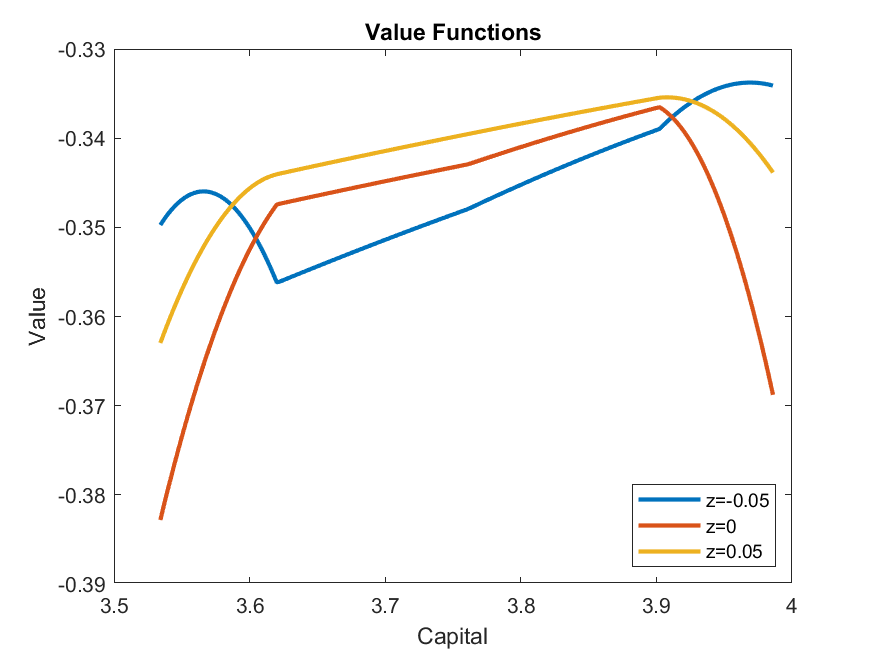
\includegraphics{econ714_homework2_question6_plot_value_functions.png}
       \caption{Value functions using finite elements}
       \label{finite_elements}
   \end{figure}
    
    \section{Deep Learning}
    
    I couldn't solve this one. I'm really sorry. I tried to follow Fernandez-Villaverde, J., Nuno, G., Sorg-Langhans, G., \& Vogler, M. (2020) and the Julia code, but I couldn't even replicate the results for the continuous time model. 
    
    \pagebreak
    \section*{References}
    
    \begin{itemize}
        \item Fernandez-Villaverde, J., Nuno, G., Sorg-Langhans, G., \& Vogler, M. (2020). Solving high-dimensional dynamic programming problems using deep learning. \textit{Unpublished working paper}.
        
        \item Heer, B., \& Maussner, A. (2008). Value function iteration as a Solution Method for the Ramsey Model.
        
        \item McGrattan, E. R. (1996). Solving the stochastic growth model with a finite element method. \textit{Journal of Economic Dynamics and Control, 20}(1-3), 19-42.
    \end{itemize}
    
  

    

%\hfill

%\pagebreak 

%\pagestyle{empty}

%\section*{Codes}


    %\begin{lstlisting}[language= R]
    
%-


    
    %\end{lstlisting}

    
    
 \end{document}
 